% !TeX spellcheck = id_ID
\documentclass[a4paper,12pt]{article}
\usepackage[bahasa]{babel}
\usepackage{graphicx}
\usepackage{multirow}
\usepackage{enumitem}
\usepackage{listings}
\usepackage{wrapfig}
\usepackage[T1]{fontenc}
\usepackage{inconsolata}
\usepackage{lipsum}

\usepackage{color}
\usepackage[table]{xcolor}
\definecolor{pblue}{rgb}{0.13,0.13,1}
\definecolor{pgreen}{rgb}{0,0.5,0}
\definecolor{pred}{rgb}{0.9,0,0}
\definecolor{pgrey}{rgb}{0.46,0.45,0.48}
\lstset{language=Java,
	showspaces=false,
	showtabs=false,
	breaklines=true,
	showstringspaces=false,
	breakatwhitespace=true,
	commentstyle=\color{pgreen},
	keywordstyle=\color{pblue},
	stringstyle=\color{pred},
	basicstyle=\ttfamily,
	moredelim=[il][\textcolor{pgrey}]{$$},
	moredelim=[is][\textcolor{pgrey}]{\%\%}{\%\%}
}

\graphicspath{ {./img/} }
\begin{document}
\title{ {\Large Laporan Praktikum}\\ Algoritma dan Pemrograman \\{\Large Pertemuan 7}}

\author{Aldzikri Dwijayanto Prathama 
	\\195410189
	\\Teknik Informatika}
\makeatletter
\begin{titlepage}
	\begin{center}
		{\huge \bfseries \@title }\\[14ex]
		
\includegraphics[scale=.8]{logo}\\[4ex]
		{\large \@author}\\[19ex]
		{\large \bfseries {SEKOLAH TINGGI MANAJEMEN INFORMATIKA DAN KOMPUTER
				AKAKOM YOGYAKARTA}}
	\end{center}


%{\large \@date} 
\end{titlepage}
\makeatother
%\maketitle
\newpage
\tableofcontents
\newpage

\section{Tujuan}
Mahasiswa dapat mengimplementasikan menyelesaikan kasus konsep perulangan while untuk
\section{Dasar Teori}
\paragraph{}
Perulangan WHILE banyak digunakan pada program yang terstruktur. Perulangan
ini banyak digunakan bila jumlah perulangannya belum diketahui. Proses perulangan
akan terus berlanjut selama kondisinya bernilai benar (true) dan akan berhenti bila
kondisinya bernilai salah.\\
Karakteristik while() adalah:
\begin{enumerate}
	\item Dilakukan pengecekan kondisi terlebih dahulu sebelum dilakukan perulangan. Jika kondisi yang dicek bernilai benar (true) maka perulangan akan dilakukan.
	\item Blok statement tidak harus ada. Struktur tanpa statement akan tetap dilakukan
	selama kondisi masih true.
\end{enumerate}
Bentuk umum :\\

\begin{lstlisting}[frame=single, linewidth=5cm]
While(ungkapan)
	Pernyataan
\end{lstlisting} 

Keterangan :
\begin{itemize}
	\item bagian pernyataan akan diekseskusi selama ungkapan dalam while bernilai benar.
	\item Pengujian terhadap ungkapan pada while dilakukan sebelum bagian pernyataan.
	\item Kemungkinan pernyataan pada while tidak dijalankan sama sekali, jika ketemu
	kondisi yang pertama kali bernilai salah.
\end{itemize}
\newpage
Flowchart perulangan while dapat dilihat seperti gambar berikut :\\
\begin{center}
	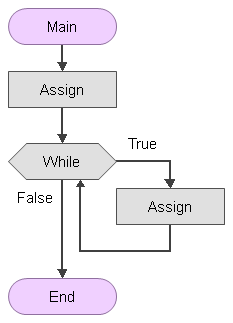
\includegraphics[scale=.5]{image--022}
\end{center}
Catatan:\\
Pernyataan perulangan dengan while akan selalu dikerjakan jika ungkapan selalu benar.
Oleh karena itu, kita harus membuat kondisi suatu saat ungkapan bernilai salah agar
perulangan berakhir.

\section{Praktik}
\subsection{Praktik 1}
\paragraph{Masalah\\}
Ketik program di bawah
\begin{lstlisting}
import java.util.Scanner;
public class UlangWhile1
{
    public static void main(String args[])
    {
        Scanner masuk = new Scanner(System.in);
        int bil;
        bil=1;
        while (bil<=5) {
            System.out.println(bil);
            bil=bil+1;
        }
    }
}
\end{lstlisting}
Buat flowchart untuk program diatas seperti berikut :\\
\begin{center}
	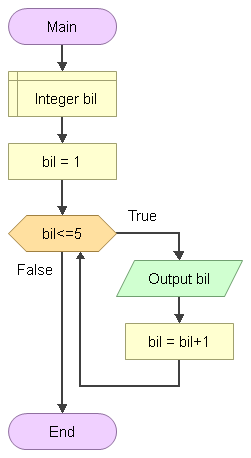
\includegraphics[scale=.5]{image--024}
\end{center}
\paragraph{Penyelesaian\\}
\begin{center}
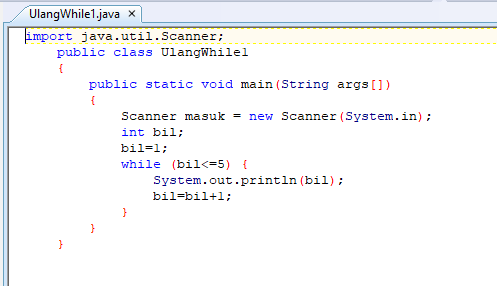
\includegraphics[width=\linewidth]{Capture1}\\
\end{center}
\newpage
\begin{center}
 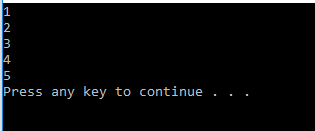
\includegraphics[scale=1]{Capture2}
\end{center}
Pada output di atas terlihat bahwa tersebut melakukan penghitungan 1 - 5, di dalam program terdapat
\begin{lstlisting}
while (bil<=5) {
            System.out.println(bil);
            bil=bil+1;
        }
\end{lstlisting}
yang mana fungsi \texttt{while} tersebut akan melakukan perulangan jika variabel \texttt{bil} memiliki nilai kurang dari sama dengan 5. Di dalam while terdapat pernyataan untuk mengeprint variabel bil, yang sebelumnya sudah diberi nilai 1, lalu akan menambahkan variabel bil dengan 1 sampai variabel bil bernilai lebih dari sama dengan 5. Maka fungsi while tersebut akan melakukan penghitungan 1 - 5.
\begin{center}
	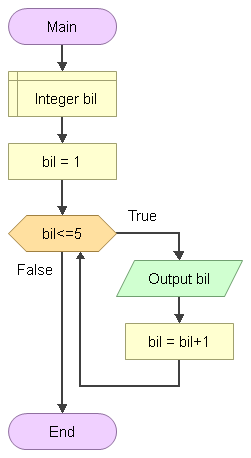
\includegraphics[scale=.5]{image--024}
\end{center}
Dari flowchart di atas terlihat jelas alur dari program sebelumnya, fungsi \texttt{while} akan melakukan pengecekan terlebih dahulu terhadap kondisi yang di berikan, pada kasus ini yaitu bil<=5, jika benar program akan mengeluarkan nilai dari variabel bil, dan menambahkannya dengan satu, lalu akan mengulanginya lagi sampai kondisi yang dicek false.

\subsection{Praktik 2}
\paragraph{Masalah\\}
Modifikasi praktik 1 dengan mengubah perrnyataan bil=1 yang ada pada baris 8
menjadi bil=5, dan pernyataan while(bil<=5) yang ada dibaris ke 9 dengan
while(bil>=1) dan bil=bil+1 pada baris 11 menjadi bil=bil-1, amati hasil outputnya,
kenapa bisa demikian, jelaskan !

\paragraph{Penyelesaian\\}
\begin{center}
	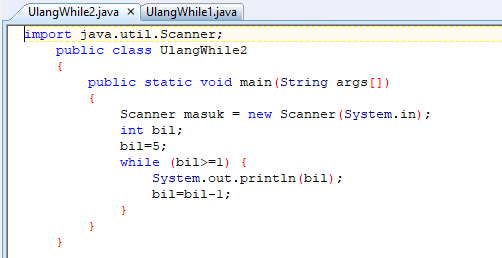
\includegraphics[width=\linewidth]{Capture4}
	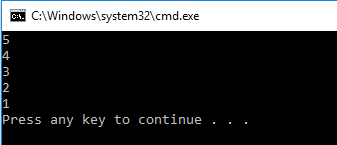
\includegraphics[scale=1]{Capture5}
\end{center}
Program menjadi menghitung mundur, itu karena nilai awal variabel \texttt{bil} adalah 5, lalu kondisi pada \texttt{while} adalah bil>=1 dengan salah satu pernyataannya \texttt{bil=bil+1}, itu berarti while akan mengurangi variabel \texttt{bil} yang bernilai 5 dengan 1 di setiap pengulangannya sampai variabel bil bernilai kurang dari sama dengan 1. 

\subsection{Praktik 3}
\paragraph{Masalah\\}
Buat program untuk menampilkan tulisan STMIK AKAKOM dan buat suatu
pernyataan jika tulisan tersebut bisa ditampilkan selama jawaban True (Ya) dan akan
di hitung jumlah yang di tampilkan
\begin{lstlisting}[frame=single, basicstyle=\small]
import java.util.Scanner;
public class modul8_3 {
    public static void main(String[] args) {
        boolean running = true;
        int counter = 0;
        String jawab;
        Scanner scan = new Scanner(System.in);
        while( running ) {
            System.out.println("STMIK AKAKOM");
            System.out.print("Tampilkan Tulisan lagi [ya/tidak]> ");
            jawab = scan.nextLine();
            // cek jawabnnya, kalau ya maka berhenti mengulang
            if( jawab.equalsIgnoreCase("tidak") ){
                running = false;
            }
                counter++;
        }
        System.out.println("Anda sudah melakukan perulangan sebanyak " + counter + " kali");
    }
}
\end{lstlisting}


\end{document}